\documentclass[12pt]{article}

\usepackage{amssymb,amsmath,amsfonts,eurosym,geometry,ulem,graphicx,caption,color,setspace,sectsty,comment,footmisc,caption,natbib,pdflscape,subfigure,array,hyperref}
\usepackage{xcolor} % for colors
\pagecolor[rgb]{0,0,0}   % dark background (near black)
\color[rgb]{0.9,0.9,0.9}       % light text (near white)

\usepackage{sectsty}
\usepackage{float}

\sectionfont{\normalsize}
\subsectionfont{\normalsize}

\usepackage[most]{tcolorbox}
\newtcolorbox{theory}[2][]{breakable,sharp corners, skin=enhancedmiddle jigsaw,
parbox=false, boxrule=0mm, leftrule=2mm, boxsep=0mm, arc=0mm, outer arc=0mm,
attach title to upper, after title={\ },
coltitle=white, coltext=white,
colback=blue!50!black, colframe=blue!80,
title={#2}, fonttitle=\bfseries, #1}

\newtcolorbox{example}[2][]{breakable,sharp corners, skin=enhancedmiddle jigsaw,
parbox=false, boxrule=0mm, leftrule=2mm, boxsep=0mm, arc=0mm, outer arc=0mm,
attach title to upper, after title={\ },
coltitle=white, coltext=white,
colback=gray!30!black, colframe=gray!70,
title={#2}, fonttitle=\bfseries, #1}

\newtcolorbox{aside}[2][]{breakable,sharp corners, skin=enhancedmiddle jigsaw,
parbox=false, boxrule=0mm, leftrule=2mm, boxsep=0mm, arc=0mm, outer arc=0mm,
attach title to upper, after title={\ },
coltitle=white, coltext=white,
colback=red!40!black, colframe=red!80,
title={#2}, fonttitle=\bfseries, #1}

\normalem

\usepackage{inconsolata}   % nice monospace font
\renewcommand{\familydefault}{\ttdefault}

\onehalfspacing
\newtheorem{theorem}{Theorem}
\newtheorem{corollary}[theorem]{Corollary}
\newtheorem{proposition}{Proposition}
\newenvironment{proof}[1][Proof]{\noindent\textbf{#1.} }{\ \rule{0.5em}{0.5em}}

\newtheorem{hyp}{Hypothesis}
\newtheorem{subhyp}{Hypothesis}[hyp]
\renewcommand{\thesubhyp}{\thehyp\alph{subhyp}}

\newcommand{\red}[1]{{\color{red} #1}}
\newcommand{\blue}[1]{{\color{blue} #1}}

\newcolumntype{L}[1]{>{\raggedright\let\newline\\arraybackslash\hspace{0pt}}m{#1}}
\newcolumntype{C}[1]{>{\centering\let\newline\\arraybackslash\hspace{0pt}}m{#1}}
\newcolumntype{R}[1]{>{\raggedleft\let\newline\\arraybackslash\hspace{0pt}}m{#1}}

\geometry{left=1.0in,right=1.0in,top=1.0in,bottom=1.0in}

\begin{document}

\begin{titlepage}
\title{{\Large Alpha extension with value and momentum factors}}
\author{{\normalsize Haeohreum Kim}\thanks{e-mail: haeohreum09@hotmail.com, independent research}}
\date{\today}
\maketitle
\begin{abstract}
\noindent {\small We explore what alpha extension strategies are, and attempt to build an alpha extension strategy 
using regress-then-rank techniques with value and momentum factors. We target the Russell 1000 index.

This paper aims to serve as an educational resource rather than a novel finding of alpha.}
\vspace{0in}\\
\noindent{\footnotesize \textbf{Keywords:} Alpha extension, value, momentum, quantitative factor investing, factor investing} \\

\bigskip
\end{abstract}
\setcounter{page}{0}
\thispagestyle{empty}
\end{titlepage}
\pagebreak \newpage

\tableofcontents

\pagebreak

\section{Overview and introduction}
\subsection{What is factor investing?}
Factor investing is characterised by the usage of multiple explanatory 'factors' in order to predict 
future returns. Generally, these factors are comprised of a mix of fundamental factors, as well as 
other market anomalies or "effects". A good example of a commonly-used effect is \textbf{momentum}, 
where past returns are thought to be indicative of future returns (Jegadeesh and Titman 1993).
\newline \\
Arbitrage pricing theory (APT) states that the expected return of some financial asset (in our case, equities)
can be expressed as a \textbf{linear} function of multiple macro-economic and/or firm-specific factors (Ross, 1976). Given
some set of factors $F = \{F_1, F_2, ..., F_p\}$, and expected returns on a given month $E(R_i)$, we have

$$ E(R_i) = \beta_0 + \sum_{i=1}^p \beta_i F_i$$
Given a portfolio of stock $S = \{S_1, S_2, \dots, S_n\}$, and their expected returns on a given month $i,$ $E(R) = \{E(R_{1i}), E(R_{2i}), \dots, E(R_{ni})\}$, we are then motivated to go long (buy) our highest
expected return stocks and short (sell) our lowest expected return stocks.
\subsection{What is alpha extension?}
\textbf{Alpha extension} is a type of fund/portfolio which is comprised of a long and short component. We 
generally state the composition of portfolios using a slash (/), such that 130/30 indicates a 130\% long 
and 30\% short component, for a net exposure of 160\%.
\newline \\ 
The easiest way to interpret alpha extension strategies that I have found, is to sepearate the portfolio
into a 100\% long, index-tracking component, and an additional 'equity market neutral' component to overlay
the passive index weights. \textbf{Equity market neutral} refers to a portfolio that is equally as short 
as it is long, and generally tracks for a low correlation to the market (a low beta).
In construction, we begin with a passive index weight (tracking the index), and then optimise for an 'alpha 
overlay' component to tilt the weights for an expected excess return.

\section{Data}
\subsection{Sources}

I sourced my data from Sharadar; specifically using 
\begin{itemize}
    \item Sharadar Core US Fundamentals
    \item Sharadar Equity Prices
\end{itemize}
As with any equity data set, I found plenty of issues in the data. I have taken care to clean data where possible - a big problem is the overstatement of market caps due to anomalous prices (for example, prices 
in the billions!). I generally filtered these stocks from our Russell 1000 proxy by using a variety 
of fundamental factors to consider nonsensical values. The remaining index appeared to adequately
track an index ETF.
\newline \\ 
Furthermore, I cannot guarantee that there is no form of data leakage in Sharadar's value factors. The results
that we see indicate to me that if there is any leakage, that it is extremely minor, as the edge we see 
is consistent with literature and also not absurd.

\section{Universe and benchmark details}

We use the Russell 1000 - the top 1000 stocks in the U.S equities market, as our benchmark. I do not have access to the actual constituents of the Russell 1000 across history; this data is expensive. Rather,
I proxied the index with a market-cap weighted ranking. I rebalanced on June every year, and shifted
the constituents to remove lookahead bias on the rebalance date.
\newline \\
I found that the proxy was a good enough representation of the index - and used the proxy as my universe + 
benchmark for the alpha extension strategy (to not cross-contaminate comparing the proxy universe to the 
actual returns of the Russell 1000).

\section{Factors}
\subsection{Value}

The idea that the value of a stock relative to the pricing of the stock and it's fundamental value is 
predictive of future returns has been a thoroughly researched topic in empirical finance. Fama and French's 
1992 paper 'The Cross-Section of Expected Stock Returns' detailed that book-to-market was significantly 
explanatory of average returns on a cross-sectional basis (Fama and French 1993).
\newline \\
At the time, this challenged the original CAPM model, which suggested that the market factor ($\beta$)
was the only explanatory factor of a stock's returns. In our data set, we have access to the following
value factors:
\begin{itemize}
    \item P/E: Price-to-equity
    \item P/B: Price-to-book
    \item P/S: Price-to-sales
    \item EV/EBITDA: Enterprise value on EBITDA
    \item EV/EBIT: Enterprise value on EBIT
\end{itemize}
An important consideration is that value factors are sector-sensitive. For example, technology stocks 
will be valued at different ratios to financial stocks. For this reason, we \textbf{sector-neutralise}
the value factors. This essentially involves z-scoring per-month, at a sector level.
\newline \\
We then consider the forward 3-month return Spearman rank correlation of each of these factors,
taking a 5-year rolling average. In factor investing, we refer to the rank correlation as the 'rank information coefficient (IC)' - which indicates the "skill" of the factor at predicting the ranks of 
the cross-sectional returns correctly. A positive rank IC indicates a better-than-guessing prediction
ability.
\begin{figure}[H]
    \centering
    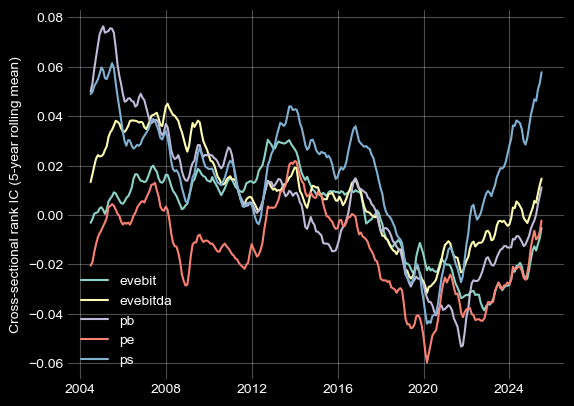
\includegraphics[width=13cm]{./static/value_factor_ic.png}
    \caption{Information coefficients (IC) of value factors over time}
    \label{fig:value_factor_ic}
\end{figure}
We can observe in Figure 1 that the value factors have moderate explanatory power pre-2018, before 
quickly degrading and then recovering post-2022. It is then observed that times of distress (even looking
at 2008) are deterimental for value factor explainability. Looking at the IC $t$-stat, we can see that 
the factors are signifcant at at 5-10\% significance level pre-2018.
\begin{theory}{IC $t$-stat} \\
    The IC $t$-stat is the time-series $t$-statistic of the
    information coefficient (IC). It measures whether the
    average correlation between factor scores and subsequent
    returns is statistically different from zero. A higher
    absolute $t$-stat indicates that the factor’s predictive
    power is more likely to be genuine rather than due to
    random noise.
\end{theory}
\begin{figure}[H]
    \centering
    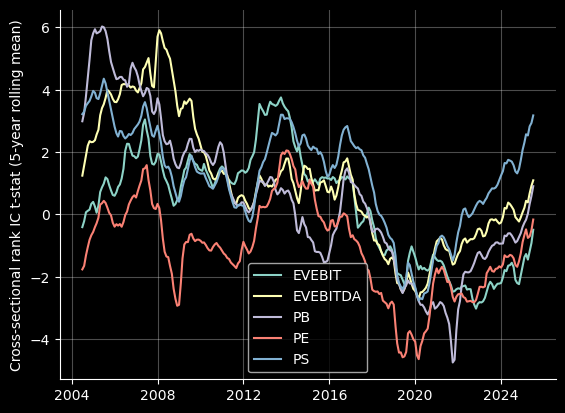
\includegraphics[width=13cm]{./static/value_factor_t_stat.png}
    \caption{IC t-stat of value factors over time}
    \label{fig:value_factor_t_stat}
\end{figure}
Across 1000 stocks, the weak-to-moderate explainability seen in our value factors is certainly enough
to deliver some alpha.
\begin{aside}{Composite factors} \\
    A common approach taken by institutional funds who have access to possibly dozens or hundreds
    of value factors (or any style of factors in general) is to take a composite. The most simple 
    method is to take the mean of all of the value factors on each time period.
\end{aside}
For our value factors, we re-center the factors cross-sectionally, for the sake of interpretability as 
well as usage in regularised linear models.

\subsection{Momentum}
Jegadeesh and Titman's 'Returns to Buying Winners and Selling Losers: Implications for Stock Market Efficiency' (1993) detailed the explanatory power of returns from 12 months prior to 2 months prior ($P_{T-12} \to P_{T-2}$) on future returns. Why skip $P_{T-2} \to P_{T-1}$? Lehmann's 'Fads, Martingales and Market Efficiency' (1990) foudn that $P_{T-2} \to P_{T-1}$ were indicative of a short-term \textbf{reversal}.
\newline \\
Therefore, the style factor of \textbf{momentum} has two separate factors - one that is indicative of 
future positive return (previous winners $\to$ future winners) and reversal.
\begin{figure}[H]
    \centering
    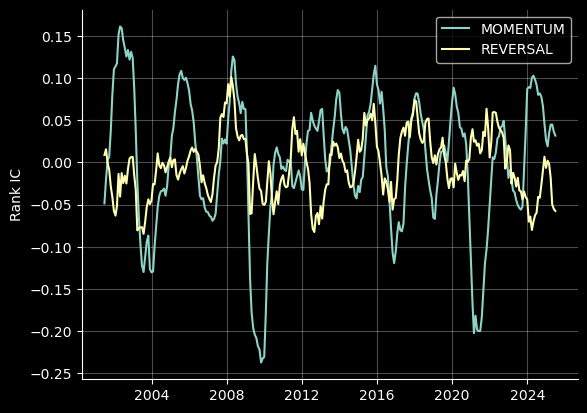
\includegraphics[width=13cm]{./static/momentum_rank_ic.png}
    \caption{Rank IC of momentum and reversal factors}
    \label{fig:momentum_rank_ic}
\end{figure}
We can observe that the reversal factor appears to point in the wrong direction (we should expect a negative 
rank IC), whereas momentum is a strong (yet transitive) predictor. We chose not to use the reversal factor 
due to our 3-month forward returns target. Momentum is \textit{not} sector-sensitive, and thus we just 
normalise the momentum factor cross-sectionally.
\newpage
\section{Portfolio and model construction}
\subsection{The alpha model}

The alpha model is constructed using Ridge penalisation. A 3-month lookback is used; with 1000 constituents 
per month, this is an estimated 3000 samples for training. This appeared to be a good sweet spot for 
not introducing too much irrelvant noise (particularly for shorter-term decay factors like momentum), and 
not enough samples\footnote{I couldn't find any authoritative information about what the actual 
optimal look-back period is. If you know more, feel free to contact me!}. The alpha model is then expressed 
by

$$ E(R) = \beta_0 + \beta_1 \cdot \texttt{EV/EBITDA} + \beta_2 \cdot \texttt{EV/EBIT} + \beta_3 \cdot \texttt{P/E} + \beta_4 \cdot \texttt{P/B} + \beta_5 \cdot \texttt{P/S}
$$

\subsection{Portfolio construction}

For simplicity sake, I used an inverse-volatility weighting for the alpha overlay. This (erroneously)
assumes that the correlation between the companies in our universe is irrelevant for the scaling of 
our weights. We take a 130/30 alpha extension strategy.
\begin{example}{Portfolio weight calculation example}
\begin{verbatim}
# long-only index tracking weights first
index_w = tst_data['index_weight']

# inverse volatility weighting
inv_vol = 1 / tst_data['volatility_est']
raw_scores = tst_data['pred_return'] * inv_vol

raw_scores = raw_scores - raw_scores.mean()
overlay_weights = 0.6 * raw_scores / raw_scores.abs().sum()

# alpha weights
alpha_w = index_w + overlay_weights
\end{verbatim}
\end{example}
You can observe in the above code snippet that we begin with the index weights, and then overlay the 
inversed-volatiltiy weights onto the index weight to get our final alpha weights.

\section{Results}
\subsection{Returns on benchmark}
\begin{figure}[H]
    \centering
    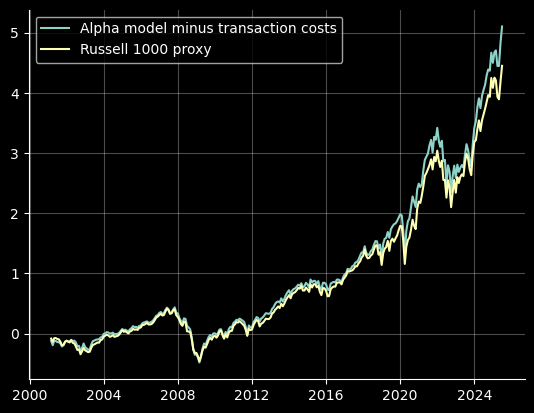
\includegraphics[width=13cm]{./static/returns.png}
    \caption{The alpha extension finds alpha over the benchmark}
    \label{fig:momentum_rank_ic}
\end{figure}
Taking a transaction cost of 5 bps per transaction (per-month), we find that the alpha model finds 
overperformance in our alpha extension strategy. Below are some statistics. Of course, we have not 
considered borrow costs (for shorts + leverage) which is significant. Further research should (and hopefully
will) include an accurate estimate of short and borrow. Consider some statistics for the model below.
\begin{table}[h!]
\centering
\begin{tabular}{l r}
\hline
\textbf{Statistic} & \textbf{Value} \\
\hline
Sharpe Ratio            & 0.51   \\
Mean Annual Return      & 8.88\% \\
Mean Annual Volatility  & 17.28\% \\
Mean Annual Alpha & 0.60\% \\
\hline
\end{tabular}
\caption{Performance statistics for the alpha extension strategy}
\label{tab:performance_stats}
\end{table}
\subsection{Factor and beta exposures}

Another interesting consideration is how the factor exposures changed over the course of the backtest. 
The ability to see what drove the model's predictions is an important detail for institutional 
funds that run quantitative equity strategies, as they are able to explain why their funds 
over/underperformed (for e.g, we were "overweight" momentum).
\begin{figure}[H]
    \centering
    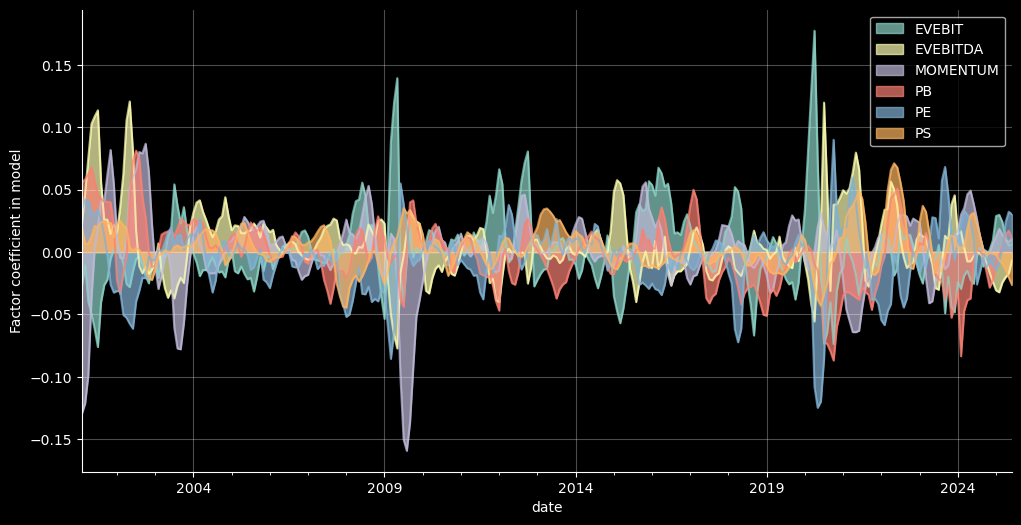
\includegraphics[width=16cm]{./static/factor_exposures.png}
    \caption{Factor exposures across history}
    \label{fig:factor_exposures}
\end{figure}
We can observe a few interesting characteristics in the above factor exposures - with the momentum factor 
inversing during the GFC crash, likely due to a largely universe-wide reversal of returns. Another interesting
period is COVID, during 2020-2021, with underweights in P/E as valuation factors break down during 
significant market downturns.
\newline \\ 
We can see that the observed alpha in our strategy is from a mix of all of our factors,
which dynamically changes throughout history. This is why having a varying set of factors is important,
as different factors are more predictive during different periods of market conditions, and explain 
different components of future returns.

\begin{figure}[H]
    \centering
    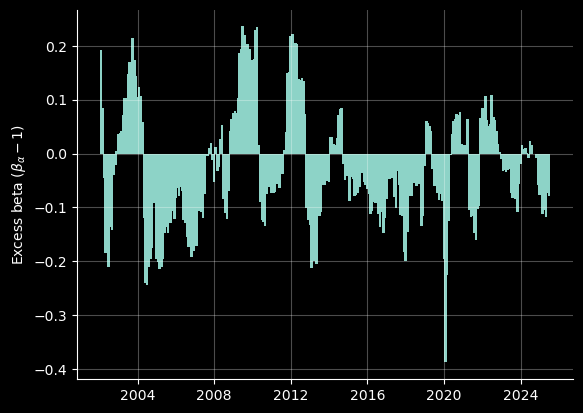
\includegraphics[width=13cm]{./static/beta_exposures.png}
    \caption{Excess beta exposure throughout history}
    \label{fig:beta_exposures}
\end{figure}

With alpha extension strategies, we generally wish to target a market beta of 1, as the alpha overlay 30/30
component is intended to be market neutral. In the above graph, we can see the "excess" beta exposure 
of our portfolio is generally around 0.8 to 0.9. If this was supposed to be an institutional fund,
this would have to likely be corrected, as pension funds/other sources of institutional money may 
expect the fund to have a 1 $\beta$ with low 'tracking error'.
\pagebreak
\section{Appendix}
\subsection{Repository of research code}

The code, databases and other auxiliary scripts used for the research in this paper can be found at this \href{https://github.com/haezera/quant-strats-in-us-equities}{\textcolor{red}{link}}.

\pagebreak
\begin{thebibliography}{}

\bibitem[Fama and French(1992)]{fama1992}
Fama, E. F., \& French, K. R. (1992).  
The Cross-Section of Expected Stock Returns.  
\textit{The Journal of Finance}, 47(2), 427–465.  
doi:\href{https://doi.org/10.2307/2329112}{10.2307/2329112}.

\bibitem[Jegadeesh and Titman(1993)]{jegadeesh1993}
Jegadeesh, N., \& Titman, S. (1993).  
Returns to Buying Winners and Selling Losers: Implications for Stock Market Efficiency.  
\textit{The Journal of Finance}, 48(1), 65–91.  
doi:\href{https://doi.org/10.1111/j.1540-6261.1993.tb04702.x}{10.1111/j.1540-6261.1993.tb04702.x}.

\bibitem[Lehmann(1990)]{lehmann1990}
Lehmann, B. N. (1990).  
Fads, Martingales, and Market Efficiency.  
\textit{The Quarterly Journal of Economics}, 105(1), 1–28.  
doi:\href{https://doi.org/10.2307/2937816}{10.2307/2937816}.

\bibitem[Ross(1976)]{ross1976}
Ross, S. A. (1976).  
The Arbitrage Theory of Capital Asset Pricing.  
\textit{Journal of Economic Theory}, 13(3), 341–360.  
doi:\href{https://doi.org/10.1016/0022-0531(76)90046-6}{10.1016/0022-0531(76)90046-6}.

\end{thebibliography}
\end{document}